\section{実行実験}\label{chap:exp}

%%%%%%%%%%%%%%%%%%%%%%%%%%%%%%
\begin{figure*}[t]
  \centering
  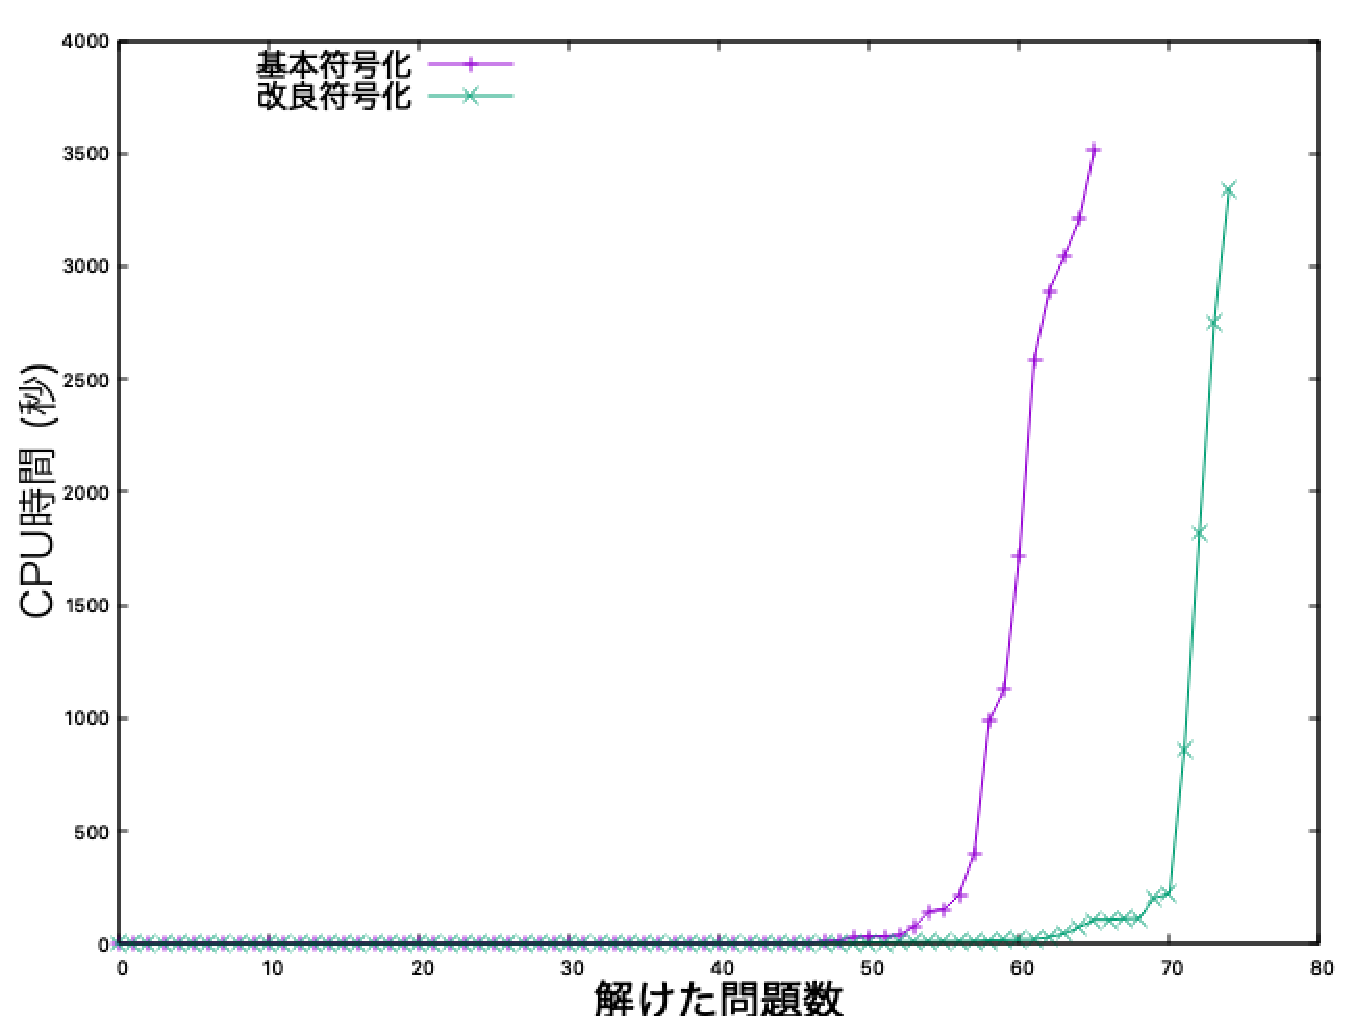
\includegraphics[scale=0.4]{fig/cactus.eps}
  \caption{基本符号化(コード~\ref{code:srf1.lp})と改良符号化(コード~\ref{code:srf2.lp})の比較} 
  \label{fig:cactus}
\end{figure*}
%%%%%%%%%%%%%%%%%%%%%%%%%%%%%%

%%%%%%%%%%%%%%%%%%%%%%%%%%%%%%
\begin{table*}[t]
  \caption{基本符号化(コード~\ref{code:srf1.lp})と改良符号化(コード~\ref{code:srf2.lp})の比較 (解けた問題数)} 
  \label{table:kibo}
  \centering
  \begin{tabular}[t]{rcr|c|cc}
    \noalign{\hrule height 1pt}
    \multicolumn{3}{c|}{辺の数} & 問題数 & 基本符号化 & 改良符号化 \\
    \noalign{\hrule height 1pt}
    %%%%%%%% 
       1 &~& 1000 & 30 & \textbf{30} & \textbf{30} \\ %\hline
    1001 &~& 4000 & 20 & \textbf{20} & \textbf{20} \\ %\hline
    4001 &~& 7000 & 11 & 9 & \textbf{10} \\ %\hline
    7001 &~& 10000 & 8 & 4 & \textbf{6}  \\ %\hline
    10001 &~& 20000 & 9 & 2 & \textbf{5} \\ %\hline
    20001 &~& 30000 & 2 & 1 & \textbf{2} \\ %\hline
    30001 &~& 40000 & 1 & 0 & 0 \\ %\hline
    40001 &~& 50000 & 4 & 0 & \textbf{2} \\
    %%%%%%%% 合計
    \noalign{\hrule height 1pt}
    \multicolumn{3}{c|}{計} & 85 & 66 & \textbf{75} \\
    \noalign{\hrule height 1pt}
  \end{tabular}
\end{table*}
%%%%%%%%%%%%%%%%%%%%%%%%%%%%%%

%%%%%%%%%%%%%%%%%%%%%%%%%%%%%%
\begin{table*}[t]
  \centering
  \caption{シングルショット符号化(コード~\ref{code:roop})とマルチショット符号化(コード~\ref{code:incmode})の比較結果}
  \label{table:trans}
  \begin{tabular}{c|r|r|r|r}  
 \noalign{\hrule height 1pt}
 問題名 & \multicolumn{1}{|c|}{ステップ長$t$} & \multicolumn{1}{|c|}{外部(sec)} 
		 & \multicolumn{1}{|c|}{ライブラリ(sec)} & \multicolumn{1}{|c}{比率} \\
 \noalign{\hrule height 1pt}
s1\_g60 & 8 & 50.098 & 25.659 & 1.952 \\
s1\_g70 & 8 & 47.177 & 24.981 & 1.889 \\
s1\_g80 & 8 & 43.193 & 15.852 & 2.725 \\
s1\_g90 & 8 & 48.984 & 22.983 & 2.131 \\
s1\_g100 & 6 & 20.964 & 4.709 & 4.452 \\
\hline
s10\_g60 & 6 & 21.947 & 5.132 & 4.277 \\
s10\_g70 & 8 & 43.840 & 16.290 & 2.691 \\
s10\_g80 & 6 & 21.156 & 4.887 & 4.329 \\
s10\_g90 & 6 & 21.276 & 5.324 & 3.996 \\
s10\_g100 & 8 & 45.704 & 17.697 & 2.583 \\
\hline
s20\_g60 & 6 & 21.202 & 4.973 & 4.263 \\
s20\_g70 & 4 & 9.890 & 2.699 & 3.664 \\
s20\_g80 & 8 & 48.473 & 16.335 & 2.967 \\
s20\_g90 & 10 & 107.938 & 64.441 & 1.675 \\
s20\_g100 & 8 & 48.473 & 17.894 & 2.709 \\
\hline
s30\_g60 & 6 & 21.189 & 5.287 & 4.008 \\
s30\_g70 & 4 & 9.901 & 2.735 & 3.620 \\
s30\_g80 & 6 & 21.884 & 5.223 & 4.190 \\
s30\_g90 & 4 & 9.979 & 2.658 & 3.754 \\
s30\_g100 & 8 & 50.344 & 18.845 & 2.671 \\
\hline
s40\_g60 & 8 & 44.637 & 14.254 & 3.132 \\
s40\_g70 & 6 & 21.334 & 4.795 & 4.449 \\
s40\_g80 & 8 & 45.202 & 14.099 & 3.206 \\
s40\_g90 & 6 & 21.710 & 5.119 & 4.241 \\
s40\_g100 & 6 & 21.299 & 5.666 & 3.759 \\
\hline
s50\_g60 & 4 & 10.021 & 2.726 & 3.676 \\
s50\_g70 & 6 & 21.291 & 4.718 & 4.513 \\
s50\_g80 & 6 & 21.163 & 6.503 & 3.254 \\
s50\_g90 & 10 & 108.299 & 65.352 & 1.657 \\
s50\_g100 & 4 & 9.934 & 2.700 & 3.679 \\
 \noalign{\hrule height 1pt}
\end{tabular}

\end{table*}
%%%%%%%%%%%%%%%%%%%%%%%%%%%%%%

提案アプローチの有効性を評価するために,
節~\ref{chap:encode}と節~\ref{chap:trans}の符号化に基づくソルバー
を開発し,実行実験を行った.

\textbf{根付き全域森問題.}
ベンチマークとしては,
DNET~\footnote{\url{https://github.com/takemaru/dnet}}
で公開されている配電網問題3問,および,
Graph Coloring and its Generalization~\footnote{\url{http://mat.tepper.cmu.edu/COLOR04/}}
で公開されているグラフ彩色問題を元に生成した82問\footnote{%
グラフ彩色問題127問の中から,連結グラフで辺の数が50,000以下である
82問を使用した.根については全ノードの1/5をランダムに選んで使用した.
}を使用した.
ベンチマーク問題(計85問)の規模は,
ノードの数11〜1406,辺の数16〜49629,根の数1〜281である.
%
ASPシステムには {\clingo}-5.4.0 (\textit{trendy})を使用し,
問題1問あたりの制限時間は1時間とした.
実験環境は,Mac mini,3.2 GHz Intel Core i7,64GB メモリである.

基本符号化と改良符号化の比較結果を
図~\ref{fig:cactus}に示す.
この図はカクタスプロットと呼ばれ,
縦軸がCPU時間,横軸が解けた問題数を表す.
グラフが下に寄るほどより高速に,右に寄るほどより多くの問題を解いたこと
を意味する.
図~\ref{fig:cactus}より,改良符号化は,基本符号化と比較して,より多く
の問題を高速に解いていることがわかる.

表~\ref{table:kibo}は,解けた問題数を,ベンチマーク問題に含まれる辺の数
で分類したものである.
改良符号化は,辺の数が40,000を超えるような問題も解けており,
大規模な問題に対する有効性が確認できた. 

\textbf{根付き全域森遷移問題.}
ベンチマークとしては,DNETで公開されている実用規模の配電網問題
(\textit{fukui-tepco},\comment{問題名も記載}ノード数:432,根ノード数:72)をベースにした.
この問題の実行可能解から,スタート初期状態を5つ,ゴール状態を6つ,
をランダムに選び,それらを組み合わせた計30問の根付き全域森遷移問題を生
成した.ASPシステムと実験環境は上と同じである.

シングルショット符号化(コード~\ref{code:roop})と
マルチショット符号化(コード~\ref{code:incmode})の比較結果を
表~\ref{table:trans}に示す.
左から順に,
問題名,
解を求めるまでのステップ長,
シングルショット符号化とマルチショット符号化のそれぞれのCPU時間(秒),
マルチショット符号化を1としたときのシングルショット符号化の比率
を示している.
マルチショット符号化は,シングルショット符号化と比較して,すべての問題
をより高速に解いており,平均で3.3倍の高速化を実現している.
これにより,根付き全域森遷移問題に対するマルチショットASP解法の優位性
が確認できた.

%%% Local Variables:
%%% mode: latex
%%% TeX-master: "paper"
%%% End:
